\documentclass[a4paper,10pt]{report}
\usepackage[utf8]{inputenc}
\usepackage{amsmath}
\usepackage{color}
\usepackage{graphicx}

\newcommand{\swift}{\textsc{swift }}
\newcommand{\eagle}{\textsc{eagle }}
\newcommand{\gadget}{\textsc{gadget-2 }}

%opening
\title{SWIFT - Theory and equations}
\author{Matthieu}
\begin{document}

\maketitle





\chapter{General properties}
\label{chap:intro}

This chapter focuses on the general description of the different objects entering the \swift code and a qualitative
description of their interactions.

\section{Particles and interactions}

The \swift code follows the model of \eagle and uses four different types of particles to represent the different
objects present in the Universe. These different types with their \gadget names are summarized in table
\ref{tab:parttypes}.

\begin{table}[h]
\centering

\begin{tabular}{|l|l|l|}
\hline
\textbf{Object} & \textbf{\gadget name} & \textbf{Description} \\
\hline
Gas & PartType0 & Particles representing the gas.\\
DM & PartType1 & Particles representing the dark matter.\\
Star & PartType4 & Particles representing the stars.\\
BH & PartType5 & Particles representing the black holes.\\
\hline
\end{tabular}
\caption{\label{tab:parttypes}The four types of particles present in the \swift code.}
\end{table}

All of these particles are affected by the gravitation force but additional interactions will exit for the non-DM
particles. The number of DM particles is a constant but the number of gas, star and BH particles will vary
over the simulation time. The latter two will typically increase while the number of gas particles will usually
decrease. \\
Depending on the exact variation of the \eagle physics used, the total number of particles will be a
constant, implying that particles will change type but none will be spawned. \\
In a typical cosmological simulation, 50\% of the particles are DM particles, 46\% are gas particles, 4\% are star
particles and less than 0.001\% are BH particles. These numbers can change slightly when doing a ``zoom'' simulation.\\

The gas particles interact through SPH forces which are computed through two loops over the neighbouring particles
(Chapter \ref{chap:SPH}). The first of these loop is over all the particles within a range $h_i$ of the particle $i$
whereas the second on is over all particles within $h_i$ and over all particles that see particle $i$ within their
search radius $h_j$. This second loop is in principle more expensive as more neighbours have to be found. \\
Gas particles also interact gravitationally and can take part in more complex \eagle interactions. The first of these
\eagle modules is the cooling  which affects the particles on an individual basis. Depending on the age of the
Universe, the chemical composition of the gas and its density, some internal energy is added or removed to the gas.
This is done by interpolating ``cooling tables'' which have been pre-computed and yield the change of energy as a
function of all the relevant quantities. This is a very cheap module in terms of computing.

The star particles (Chapter \ref{chap:stars}) are created from gas particles when the right gas density and pressure
criteria are met. This does not require any loop over neighbours as it is a particle by particle effect. Depending on
the options chosen, a gas particle can be transformed into a star particle or it can spawn one or more star particles.\\
Once they have been created, these star particles cease to interact via SPH forces and only obey the gravity forces. \\
The star particles evolve with time in order to reflect the change in chemical element composition of their cores.
They dispatch elements to their gas neighbours through a loop of the same kind than the 1st SPH loop. There are in fact
two loops performed, one to compute the weights of the neighbours and the second one to actually dispatch the elements
and the mass. This is called ``enrichment''\\
Finally, star particles also do feedback in the form of a packet of thermal energy given randomly to one of their
neighbours. This process occurs only once in the lifetime of the star, shortly after its creation. The calculation of
the weights in the enrichment parts is useful here as well. In the latest \eagle version, the amount of energy
dispatched is a function of the velocity spread of the DM particles surrounding the star. This quantity is computed
using, once again, a loop over the neighbours. \\


The Black Hole particles (Chapter \ref{chap:BHs}) are created from gas particles when they hit the bottom of a potential
well of a given depth. These particles will then do feedback in the same way that stars do it, i.e. by dumping a certain
amount of energy to one or more neighbouring gas particles. The black hole also swallows (i.e. destroys) gas particles
passing by under some circumstances. This is achieved in the same loop over the neighbouring gas particles. There is no
interaction between the BHs and the stars or DM particles. \\

In summary, the various loops over different particles can be written in a short table (\ref{tab:interactions}). The
exact equations happening in these loops are given in the corresponding sections of this document.

\begin{table}[!h]
\centering
\begin{tabular}{|l|c|c|c|c|}
\hline
$ \nearrow$&\textbf{DM} & \textbf{Gas} & \textbf{Stars} & \textbf{BHs} \\
\hline
\textbf{DM} &  &  &  &\\
\hline
\textbf{Gas} & \textbullet & \textbullet & &\\
\hline
\textbf{Stars} &\textbullet & \textbullet & &\\
\hline
\textbf{BHs} & & \textbullet& &\\
\hline
\end{tabular}
\label{tab:interactions}
\caption{\label{tab:interactions}The various loops over neighbours required by the \eagle model. For instance, gas
particles are looping over
their gas neighbours and (in another loop) over their DM neighbours. This table does not show the frequency of the
loops. Only the gas-gas loop occurs at every time step.}
\end{table}

\section{A typical time step}

All the different particles are arranged according to their time step size in different bins and the code will then
evolve all particles in a given bin and then move to the next one. For a given set of active particles, the time step
can be decomposed as follows:

\begin{enumerate}
 \item Compute next time step.
 \item First kick for active particles.
 \item Drift (active and inactive) particles.
 \item Predict inactive particles forward in time.
 \item Compute gravity accelerations for all particles.
 \item *Compute SPH accelerations for gas particles.
 \item Calculate the cooling for the gas particles. \eagle
 \item Second kick for the active particles.
 \item Create star particles if needed. \eagle
 \item *Calculate the star's smoothing length. \eagle
 \item Evolve stars' chemical content. \eagle
 \item *Calculate the DM velocity dispersion for star particles. \eagle
 \item *Calculate the weights used for the star feedback. \eagle
 \item *Perform star feedback on gas particles. \eagle
 \item *Perform stellar enrichment. \eagle
 \item *Swallow gas particles into BH particles. \eagle
 \item Merge BH particles that lie close-by. \eagle
 \item *Perform BH feedback on gas particles. \eagle
 \item Find halos. \eagle
\end{enumerate}

The details of these individual steps are described in the next chapters. The lines post-fixed with the term \eagle are
specific of our implementation. The other elements are part of the standard \gadget code. Lines pre-fixed by an asterisk
are the loops described in the previous section and table \ref{tab:interactions}. Apart from gravity, halo finding and
the loops, all operations are performed on a particle-by-particle basis and are thus very cheap. Halo finding is only
performed very rarely and is described in chapter \ref{chap:FOF}.

\section{Units used in the code}

\textcolor{red}{To be written down.}









% ##################################################################################################################



\chapter{Dark Matter particles}
\label{chap:DMs}

This section describes the physics of the DM particles but as all particles are affected by gravity, the equations
apply to all four types. 


\section{Particle definition}
Every particle contains the following information:

\begin{table}[h]
\centering
\begin{tabular}{|l|c|l|}
 \hline
 \textbf{Quantity}  & \textbf{Symbol} & \textbf{Units} \\
 \hline \hline
 Position & $\vec{x}$ & $[m]$ \\
 Velocity &$\vec{v}$ & $[m\cdot s^{-1}]$ \\
 Acceleration &$\vec{a}$ & $[m\cdot s^{-2}]$ \\
 Mass & $m$ & $[kg]$ \\
 Softening length & $\epsilon$ & $[m]$ \\
 Time step & $\Delta t$ & $[s]$ \\
 Norm of old acceleration & $a_{old}$ & $[m\cdot s^{-2}]$ \\
\hline
\end{tabular} 
\end{table}


In what follows, we will use $\vec{r}_{ij} = \vec{x_i} - \vec{x_j}$ and $\hat{r}_{ij} = \vec{r}_{ij}/|\vec{r}_{ij}|$
to simplify the notation.\\
In most calculations, the mass and softening length of the particles are constants for a given type of particles but
this is not true anymore when including the \eagle physics as the gas, star and BH particles will change mass over
time. In cosmological simulations, the softening length is a function of time.

\section{Gravity interactions}

The gravity interactions are split in two parts, the sort range interactions computed via the FMM method and the long 
range interactions computed through a PM scheme. Short range interactions are also soften on a scale $\epsilon$ to 
reduce the effect of spurious two-body relaxation. For implementation purposes, we define the quantity $h_c = 
2.8\epsilon$, the radius at which the force becomes purely Newtonian and is not soften any more.

\begin{equation}
 \vec{a} = \vec{a}_{short} + \vec{a}_{long}
\end{equation}


The short range force is computed thanks to FMM. The expression for the acceleration of a particle $i$ due to a body 
(particle or monopole) $j$ is given by:

\begin{equation}
 \vec{a}_{short} = G\cdot f \cdot f_{LR} \cdot \vec{r}_{ij},
\end{equation}
 where $G$ is Newton's constant, $f$ is the softened local force and $f_{LR}$ is the correction factor coming from the use of the mesh for long distance forces.
 The softened local force is 

\begin{equation}
\nonumber
 f = \left\lbrace \begin{array}{rcl}
                    \frac{1}{|\vec{r}_{ij}|^3}  & \mbox{if} & |\vec{r}_{ij}| > h_c\Big. \\
                    \frac{1}{h_c^3}\left(-\frac{32}{3}\frac{|\vec{r}_{ij}|^3}{h_c^3} + \frac{192}{5}\frac{|\vec{r}_{ij}|^2}{h_c^2} - 48\frac{|\vec{r}_{ij}|}{h_c} + \frac{64}{3} - \frac{2h_c^3}{3|\vec{r}_{ij}|^3} \right)  & \mbox{if} & h_c \geq |\vec{r}_{ij}| > \frac{h_c}{2}\Big. \\	
                    \frac{1}{h_c^3}\left(32\frac{|\vec{r}_{ij}|^3}{h_c^3} - \frac{192}{5}\frac{|\vec{r}_{ij}|^2}{h_c^2} + \frac{32}{3}\right)  & \mbox{if} & |\vec{r}_{ij}| \leq \frac{h_c}{2}\Big. \\		
		    \end{array}\right.
\end{equation}

The correction factor introduced by the long range force calculation is dependant on the parameter $r_s$, the spatial scale of the force-split.

\begin{equation}
 f_{LR} = \text{erfc}\left(\frac{|\vec{r}_{ij}|}{2r_s}\right) + \frac{|\vec{r}_{ij}|}{r_s\sqrt{\pi}}\exp\left(-\frac{|\vec{r}_{ij}|^2}{4r_s^2}\right)
\end{equation}

In practice, $r_s$ is given as a multiple ($\sim 1.25$) of the FFT-mesh size (See below). Figure \ref{fig:short_range_correction} shows the value of $f_{LR}$ for various distances $r$ (expressed in units of $r_s$.
As can be seen for distances greater than a few $r_s$, the value drops below $10^{-2}$, effectively suppressing the force contributions coming from the tree for large distances. In practice, a
cut-off distance of $r_c$ is used above which no tree interaction is performed. A choice of $r_c=4.5r_s$ is standard. Notice than in practice $r_s \gg \epsilon$.\\
The values of $r_s$ and $r_c$ are both given at compile time. \\

\begin{figure}
\centering
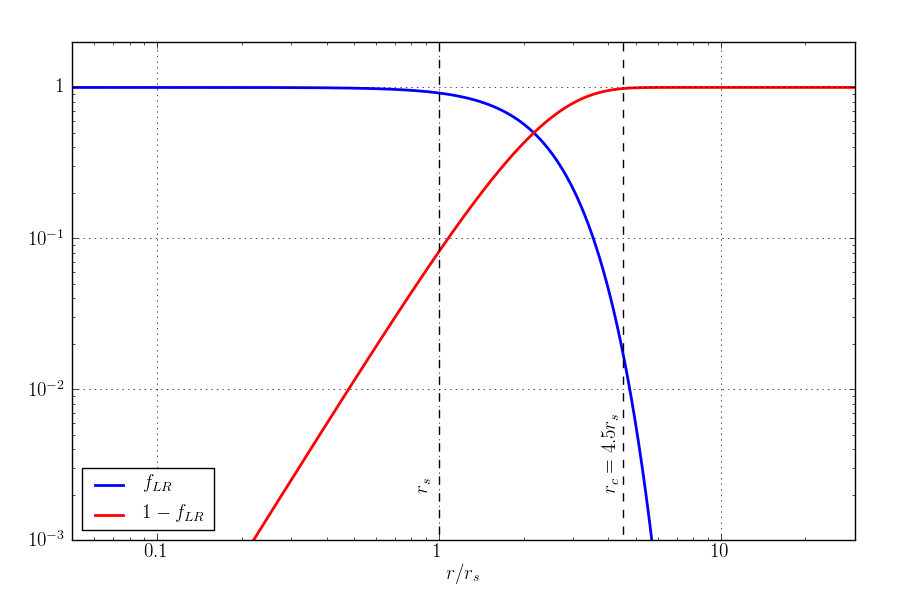
\includegraphics[width=\textwidth]{Figures/Gravity/correction}
\caption{Correction terms to the force computed from the tree due to the use of a mesh for long range forces. For distances above $r_c$, the contribution of the tree becomes neglectable and can safely be ignored.
The red curve is the complement to one of $f_{LR}$ and shows that this term only matters in a small region around $r_s$ and can safely be replaced by $1$ for $r\ll r_s$.} 
 \label{fig:short_range_correction}
\end{figure}

A similar cut-off radius could be used to avoid computing $f_{LR}$ for small $r$ (i.e. when the term is $1$). \gadget pre-computes the values of $f_{LR}$ and stores the results
in a table. This allows to avoid the expensive calculation of the exact term. \\

The long range force is computed using the FFT algoritm. In the first step, the particles are sampled on the grid to give the density field $\rho(\vec{x})$. We then use a Fourier
transform to compute the field $\hat\rho(\vec{k})$. We then compute the potential in Fourier space by applying the filter function corresponding to the term $f_{LR}$. This reads:

\begin{equation}
 \hat\phi(\vec{k}) = - \frac{4\pi G\hat\rho(\vec{k})}{|\vec{k}|^2} \exp\left(-|\vec{k}|^2 r_s^2\right).
\end{equation}

This is then transformed back to real space using an inverse FFT. The force applied to each particle is obtained by finite-differentiating this using a standard stencil:

\begin{equation}
 \frac{d\phi}{dx_i} = \frac{1}{\Delta x}\left(\frac{1}{12}\phi_{i-2,j,k} - \frac{2}{3}\phi_{i-1,j,k} + \frac{2}{3}\phi_{i+1,j,k} - \frac{1}{12}\phi_{i+2,j,k}\right)
\end{equation}

Figure \ref{fig:total_force} shows the total acceleration as a function of distance and the different contributions. The total error made in the calculation is displayed on figure
\ref{fig:total_error}. The error comes from the truncation of the short-range tree forces at a distance $r_c$. For $r_c>4.5r_s$, the error is less than $2\%$. Higher values of
$r_c$ would improve the accuracy but lead to more intereactions computed via the tree instead of via the mesh.\\

\begin{figure}
\centering
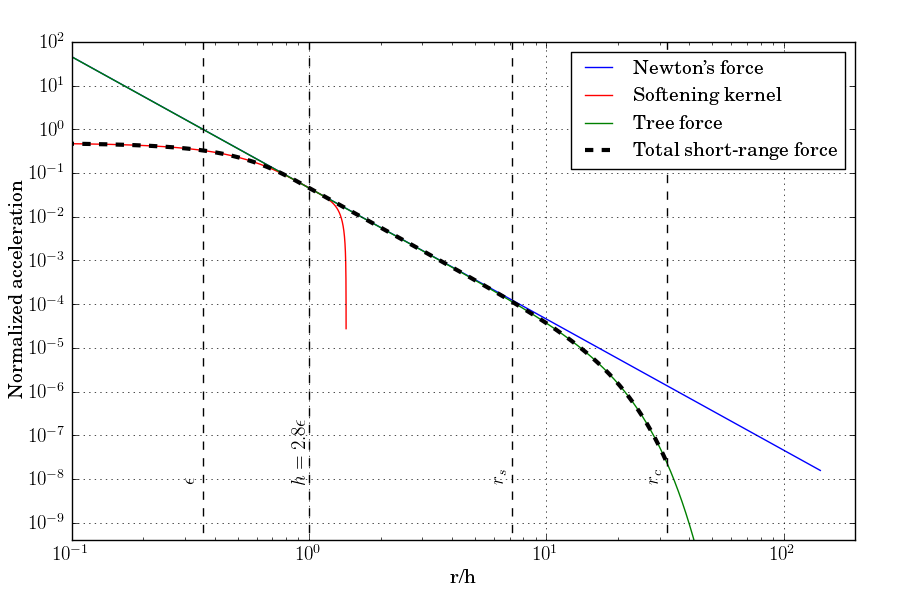
\includegraphics[width=\textwidth]{Figures/Gravity/force}
\caption{Total acceleration and the various contributions as a function of the distance $r$ in units of $h_c$. No tree-based interaction is computed for $r>r_c$.
The value of $r_s$ chosen here is arbitrary.} 
 \label{fig:total_force}
\end{figure}

\begin{figure}
\centering
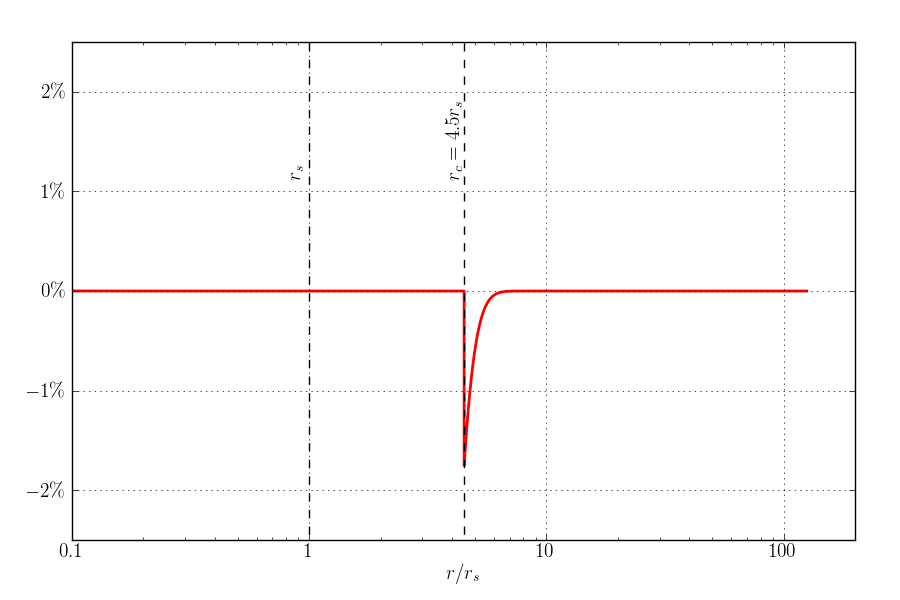
\includegraphics[width=\textwidth]{Figures/Gravity/error}
\caption{Relative error made on the acceleration calculation as a function of the distance $r$ expressed in uits of $r_s$. The error is maximal at $r=r_c$ and is less than $2\%$ in magnitude if 
one chooses $r_c > 4.5 r_s$.} 
 \label{fig:total_error}
\end{figure}

The maximal time step a particle is allowed to have is related to the acceleration by:

\begin{equation}
 \Delta t_i = \sqrt{\frac{2\eta \epsilon}{|\vec{a_i}|}}
\end{equation}

where $\eta$ is some accuracy constant which generally takes a value around $\eta \approx 0.025$.

% \section{Periodic boundary conditions}
% 
% In most cases, the simulations are run with periodic boundary conditions. The simplest way to treat the formally
% infinite number of interactions in a tree code is to use the Ewald summation technique. In this case, the acceleration
% of a particle gets a new term:
% 
% \begin{equation}
%  \vec{a_i} = \vec{a_i} + \sum_j m_j \vec{f}_c(\vec{r}_{ij}).
% \end{equation}
% 
% The correction terms $\vec{f}_c$ are expensive to compute but are constant in time and only depend on the distance
% between the particles. This means that the values can be pre-computed and stored in a table. A simple 3D interpolation
% of the values in this table is then used when actually computing the force. \gadget and other code use a $N_e=64$
% elements per dimension table representing one octant. The other ones can be obtained thanks to the symmetry properties
% of the terms. \\
% 
% The table is computed as follows. For every element $i <N_e, j<N_e,k<N_e$, we compute the vector $\vec{x} =
% (\frac{i}{2N_e}, \frac{j}{2N_e}, \frac{k}{2N_e})$. The table element $(i,j,k)$ is then:
% 
% \begin{eqnarray*}
%  \vec{E}_{ijk} &=& \frac{1}{L^2}\frac{\vec{x}}{|\vec{x}|} \\
%          & & -\frac{1}{L^2}\sum_{n_x=-l_n}^{l_n}\sum_{n_z=-l_n}^{l_n}\sum_{n_z=-l_n}^{l_n}
% \frac{\vec{x}-\vec{n}}{|\vec{x}-\vec{n}|}\left[\mathrm{erfc}\left(\alpha|\vec{x}-\vec{n}|\right) +
% \frac{2\alpha}{\sqrt{\pi}}|\vec{x}-\vec{n}|\cdot e^{-\alpha^2|\vec{x}-\vec{n}|^2}\right]\\
%          & & -\frac{1}{L^2}\sum_{h_x=-l_h}^{l_h}\sum_{h_z=-l_h}^{l_h}\sum_{h_z=-l_h}^{l_h} 2\frac{\vec{h}}{|\vec{h}|^2}
% \cdot e^{-\pi^2|\vec{h}|^2} \cdot \sin\left(2\pi\cdot \vec{h}\cdot\vec{x}\right)
% \end{eqnarray*}
% 
% where $L$ is the size of the box, $\alpha$ is an arbitrary number and the vectors $\vec{n}$ and $\vec{h}$ are defined
% as $\vec{n} = (n_x,n_y,n_z)$ and $\vec{h} = (h_x,h_y,h_z)$. \gadget uses $\alpha=2$ and $l_n=l_h=4$. The higher these
% last two values and $N_e$ are, the better the approximation. The result does not depend on $\alpha$ but depending on
% the value, the convergence of the serires toward the exact solution can vary. \\
% These tables are computed at the start of the simulation or read from a file to speed-up initialization. \\
% 
% Once the table has been computed, the values can be used to get the corrections $\vec{f}_c(\vec{r}_{ij})$.
% 
% \begin{equation}
%  \vec{f}_c(\vec{r}_{ij}) = \vec{E}_{abc}
% \end{equation}
% 
% where the indices $a$, $b$ and $c$ are rounded down integer values $(a,b,c) = \left\lfloor\frac{2N}{L}
% \vec{r}_{ij}\right\rfloor$ of the distance between particle $i$ and $j$.

% \section{Fast Multipole Method}
% 
% 
% \textcolor{red}{To be done.}






% ##################################################################################################################

\chapter{Gas particles - SPH}
\label{chap:SPH}

This chapter presents the equations used to simulate gas interactions.

\section{Particle definition}
Every particle contains the following information:

\begin{table}[h]
\centering
\begin{tabular}{|l|l|c|l|}
 \hline
 \textbf{Quantity} & \textbf{Type} & \textbf{Symbol} & \textbf{Units} \\
 \hline \hline
 Position & Primary & $\vec{x}$ & $[m]$ \\
 Velocity & Primary &$\vec{v}$ & $[m\cdot s^{-1}]$ \\
 Acceleration & Tertiary &$\vec{a}$ & $[m\cdot s^{-2}]$ \\
 Mass & Primary &$m$ & $[kg]$ \\
 Density & Secondary & $\rho$ & $[kg\cdot m^{-3}]$ \\
 Pressure & Secondary & $P$ & $[kg \cdot m^{-1}\cdot s^{-2}]$ \\
 Internal energy per unit mass & Primary & $u$ & $[m^2 \cdot s^{-2}]$ \\ 
 Energy derivative & Tertiary & $\frac{du}{dt}$ & $[ m^2 \cdot s^{-3}]$ \\
 Correction term & Secondary & $\Omega$ & $[-]$ \\
 Smoothing length & Secondary &$h$ & $[m]$ \\
 Smoothing length derivative & Tertiary &$\frac{dh}{dt}$ & $[m\cdot s^{-1}]$ \\
 Time step & Secondary & $\Delta t$ & $[s]$ \\
 Signal velocity & Secondary & $v_{sig}$& $[m\cdot s^{-1}]$ \\
\hline
 Velocity curl & Secondary & $\nabla\times \vec{v}$ & $[s^{-1}]$ \\
 Velocity divergence & Secondary & $\nabla\cdot \vec{v}$ & $[s^{-1}]$ \\
 Balsara switch & Secondary & $f$ & $[-]$ \\
\hline
\end{tabular} 
\end{table}

Secondary quantities are computed from the primary one in a loop (density loop) over all particle neighbours. Tertiary
ones are computed from secondary ones in another loop (force loop). \\

For optimisation purposes, any function of these quantities could be stored. For instance, $1/h$ instead of $h$ or
$\frac{P}{\rho\Omega}$ instead of $\Omega$ may be options worth exploring. \\

\section{Kernel function}

The kernel function can always be decomposed as:

\begin{equation}
 W(\vec{x}, h) = \frac{1}{h^3}f\left(\frac{|\vec{x}|}{h}\right) 
\end{equation}

where $f(q)$ is a low-order polynomial. The simplest possible choice is the cubic-spline kernel which (in 3D) reads
\begin{eqnarray*}
 f(q) &=& \frac{1}{\pi}\left\lbrace \begin{array}{rcl}
                      \frac{1}{4}(2-q)^3 - (1-q)^3 & \mbox{if} & 0 \leq q < 1 \\
		      \frac{1}{4}(2-q)^3 & \mbox{if} & 1 \leq q < 2 \\
		      0 & \mbox{if} & q \geq 2 \\
                     \end{array}
 \right. \\
&=&\left\lbrace \begin{array}{rcl}
    0.31831 -0.477465 q^2+0.238732 q^3& \mbox{if} & 0 \leq q < 1 \\
   0.63662 -0.95493 q+0.477465 q^2-0.0795775 q^3  & \mbox{if} & 1 \leq q < 2 \\
		      0 & \mbox{if} & q \geq 2 \\
                     \end{array}
 \right.
\end{eqnarray*}

The constants here are NOT the constants used in GADGET as we are not following their convention of setting $h$ as the
cut-off value of $W$.\\
Notice that the kernel goes to $0$ when $|\vec{r}_{ij}| = 2h$ in this case. The constant in front of $h$ depends on the
kernel
chosen and to keep it general, we should insert a constant here and say that the interaction only takes place if
$r<\zeta h$ and keep $\zeta$ as a modifiable (compile time) constant. In other words, we can say that $W(x,h)$ is a
function that goes to $0$ if $x > \zeta h$. \\
Coming back to the simplest case, the derivatives of the kernel function are given by:

\begin{eqnarray*}
 \vec\nabla_x W(\vec{x},h) &=& \frac{1}{h^4}f'\left(\frac{|\vec{x}|}{h}\right) \frac{\vec{x}}{|\vec{x}|} \\
 \frac{\partial W(\vec{x},h)}{\partial h} &=&- \frac{1}{h^4}\left[3f\left(\frac{|\vec{x}|}{h}\right) + 
\frac{|\vec{x}|}{h}f'\left(\frac{|\vec{x}|}{h}\right)\right]
\end{eqnarray*}

with

\begin{eqnarray*}
  f'(q)&=& \frac{1}{\pi}\left\lbrace \begin{array}{rcl}
                      3 \left(1-q\right)^2-\frac{3}{4} \left(2-q\right)^2 & \mbox{if} &
0 \leq q < 1 \\
 		      -\frac{3}{4} \left(2-q\right)^2 & \mbox{if} & 1 \leq q < 2 \\
		      0 & \mbox{if} & q \geq 2 \\
                     \end{array}
 \right. \\
&=&\left\lbrace \begin{array}{rcl}
    -0.95493 q + 0.716197 q^2& \mbox{if} & 0 \leq q < 1 \\
   -0.95493+0.95493 q-0.238732 q^2  & \mbox{if} & 1 \leq q < 2 \\
		      0 & \mbox{if} & q \geq 2 \\
                     \end{array}
 \right.
\end{eqnarray*}

In summary, the SPH method uses a low order polynomial $f(q)$ which vanishes for any $q>\zeta$. Those two ``objects''
are linked together and are likely to be changed in different versions of the code. It would be great to be able to
change this without really touching the code. 
Having a compilation option somewhere which activates a given form of $f$ and changes the value of $\zeta$ accordingly
would be great.

\section{First SPH loop (density)}
\label{sec:density}

In the first loop of the algorithm, the secondary quantities of particle $i$ are computed from the primary ones in the
following way:

\begin{eqnarray}
 \rho_i &=& \sum_j m_j W(\vec{r}_{ij}, h_i)\\
 h_i &=& \eta \left(\frac{m_i}{\rho_i} \right)^{1/3}
\end{eqnarray}

where $\eta \approx 1.2$ is a constant. These two equations can be solved iteratively using a Newton-Raphson or
bisection scheme. In practice, the loop is performed over all particles $j$ which are at a distance
$|\vec{r}_{ij}|<\zeta
h$ from the particle of interest. One has to iterate those two equations until their outcomes are stable.\\
Another measure of the accuracy of $h$ is the weighted number of neighbours which (in 3D) reads

\begin{equation}
 N_{ngb} = \frac{4}{3}\pi \left(\zeta h\right)^3 \sum_j W(\vec{r}_{ij},h_i)
\end{equation}

One then change $h$ until an optimal value for $N_{ngb}$ is reached. GADGET uses a bisection algorithm to do so.
The (magical) value of $N_{ngb}$ to obtain is a numerical parameter and its value can be expressed as a function of the
more physically relevant parameter $\eta$. In 3D the relation between those quantities is

\begin{equation}
 N_{ngb} = \frac{4}{3}\pi\left(\zeta \eta\right)^3
\end{equation}

We usually use $N_{ngb} = 48$, which corresponds to a sub-optimal value of $\eta=1.127$. The optimal value should be
$N_{ngb}=57.9$ ($\eta=1.2$) but this is computationally more expensive and the improvement over $N_{ngb}=48$ is not
obvious.\\ 

To increase the convergence rate, one can use the derivative of the density with respect to the smoothing length in the
Newton iterations:

\begin{equation}
 \frac{\partial \rho}{\partial h} = \sum_j m_j \frac{\partial W(\vec{r}_{ij},h_i)}{\partial h}
\end{equation}

This can also give a convergence criterion as this term must be $0$ when the right value oh $h$ has been found.
The derivative of the kernel function has to be computed anyway to obtain a value for the correction term $\Omega_i$.
This term is given by

\begin{equation}
  \Omega_i = 1 + \frac{h_i}{3\rho_i}\sum_j m_j\frac{\partial W(\vec{r}_{ij},h_i)}{\partial h}
\end{equation}

This concludes the first SPH loop in the standard implementation. More complicated quantities such as
$\vec\nabla\times\vec v_i$ or $\vec\nabla\cdot\vec v_i$ are sometimes computed here if they are needed in the force
loop.

\section{Second SPH loop (forces)}
\label{sec:forces}

Once those quantities have been obtained, the force estimation loop can be started.
First, the pressure has to be evaluated evaluated using the equation of state

\begin{equation}
\label{eq:pressure}
 P_i = \rho_i u_i (\gamma - 1)
\end{equation}

where $\gamma$ is the polytropic index. Usually, $\gamma = \frac{5}{3}$. The speed of sound in the particle is then
obtained using

\begin{equation}
 c_i = \sqrt{\frac{\gamma P_i}{\rho_i}} = \sqrt{\gamma (\gamma-1)u_i}.
\end{equation}

The second loop is used to compute the accelerations (tertiary quantities). The exact expressions are

\begin{eqnarray}
 \vec{a_i} &=& - \sum_j m_j\left[\frac{P_i}{\Omega_i\rho_i^2}\vec{\nabla_r} W(\vec{r}_{ij}, h_i) +
\frac{P_j}{\Omega_j\rho_j^2}\vec{\nabla_r}W(\vec{r}_{ij}, h_j) \right] \label{eq:acceleration}\\
 \frac{du_i}{dt} &=& \frac{P_i}{\Omega_i\rho_i^2} \sum_j m_j
(\vec{v_i}-\vec{v_j})\cdot\vec{\nabla_r} W(\vec{r}_{ij}, h_i)
\label{eq:dudt}\\
 \frac{dh_i}{dt} &=& \frac{h_i}{3}\sum_j \frac{m_j}{\rho_j} \left(\vec{v_j} - \vec{v_i} \right)
\cdot\vec{\nabla_r}W(\vec{r}_{ij}, h_i)\\
 v_{sig,i} &=& c_i + c_j + \max_j(0, 3\hat{r}_{ij} \cdot (\vec{v}_j - \vec{v}_i)) \label{eq:sigvel}
\end{eqnarray}

In practice the loop is here performed over all pairs of particles such that $|\vec{r}_{ij}| < \zeta h_i$ or
$|\vec{r}_{ij}| < \zeta
h_j$. In general, the equations are more involved as they will contain terms to mimic the effect of viscosity or
thermal conduction. These terms are pure functions of the properties of particles $i$ and $j$ and are thus very simple
to insert once the code is stabilised.\\

The time step is given by the Courant relation where the cell size is the smoothing length and the velocity is the
signal speed:

\begin{equation}
 \Delta t_i = C_{CFL} \frac{2h_i}{v_{sig,i}}.
\label{eq:dt}
\end{equation}

The Courant parameter ($C_{DFL}$)usually takes a value between $0.2$ and $0.3$. The integration in time can then
take place. The
leapfrog integrator is usually used as it behaves well when coupled to gravity. \\
In the case where only one global time step is used for all particles, the minimal time step of all particles is reduced
and used. \\

Notice that $h$ has to be recomputed through the iterative process
presented in the previous section at every time step. The time
derivative of the smoothing length only gives a rough estimate of its
change. It only provides a good guess for the Newton-Raphson (or
bisection) scheme.

\section{Time integration}

The usual scheme uses a kick-drift-kick leap-frog integrator. The various sub-steps are:

\textbf{First kick} Kick the particle for the first half-step.

\begin{eqnarray*}
 v_i^{n+1/2} &=& v_i^{n} + \frac{1}{2} a_i^{n}\Delta t^n \\
 u_i^{n+1/2} &=& u_i^{n} + \frac{1}{2} \frac{du_i^n}{dt}\Delta t^n \\
\end{eqnarray*}

\textbf{Particle drift} Advance particles by a full step

\begin{equation*}
 x_i^{n+1} = x_i^n + v_i^{n+{1/2}} \Delta t^n
\end{equation*}

\textbf{Prediction} Predict particles forward in time according to their old ``accelerations''

\begin{eqnarray*}
 v_{i,pred} &=& v_{i,pred} + a_i^{n} \Delta t^n \\
  u_{i,pred} &=& u_{i,pred} \cdot \exp\left(\frac{1}{u_i^n}\frac{du_i^{n}}{dt} \Delta t^n\right)\\
 \rho_i^{n+1} &=& \rho_i^n \cdot \exp\left(\frac{-3}{h_i^n}  \frac{dh_i^{n}}{dt} \Delta t^n \right) \\
  h_i^{n+1} &=& h_i^n \cdot \exp\left(\frac{1}{h_i^n}  \frac{dh_i^{n}}{dt} \Delta t^n \right)   \\
  \Omega_i^{n+1} &=& \Omega_i
\end{eqnarray*}

\textbf{SPH loop 1} Correct $\rho_i^{n+1}$, $h_i^{n+1}$ and $\Omega_i^{n+1}$ if needed using bisection algorithm and the
first SPH loop (Section \ref{sec:density}). \\

\textbf{SPH loop 2} Compute $a_i^{n+1}$, $\frac{du_i^{n+1}}{dt}$ and $\frac{dh_i^{n+1}}{dt}$ using the second SPH
loop (Section \ref{sec:forces}). This loop is ALWAYS performed using the PREDICTED velocity $v_{i,pred}$ and internal
energy $u_{i,pred}$ for BOTH particles. \\

\textbf{New time step} Calculate the next time step.

\begin{equation*}
 \Delta t^{n+1} = C_{CFL} \frac{2h_i}{v_{sig,i}}
\end{equation*}


\textbf{Gravity} Compute accelerations due to gravity. \\

\textbf{Cooling} Compute the change in internal energy due to radiative cooling and heating. \\

\textbf{Second kick} Kick the particle for the second half-step.

\begin{eqnarray*}
 v_i^{n+1} &=& v_i^{n+1/2} + \frac{1}{2} a_i^{n+1}\Delta t^{n} \\
 u_i^{n+1} &=& u_i^{n+1/2} + \frac{1}{2} \frac{du_i^{n+1}}{dt}\Delta t^{n} \\
 v_{i,pred} &=& v_i^{n+1} \\
 u_{i,pred} &=& u_i^{n+1} \\
\end{eqnarray*}



% A full time step of size $\Delta t$ consists of the
% following sub-steps: \\
% 
% \textbf{First kick} Compute velocity and internal energy at half step.
% 
% \begin{eqnarray*}
%  \vec{v}_i^{n+1/2} &=& \vec{v}_i^n + \textstyle\frac{1}{2}\Delta t^n ~\vec{a}_i\big|^{n-1/2} \\
%  u_i^{n+1/2} &=& u_i^n + \textstyle\frac{1}{2}\Delta t^n ~\frac{du_i}{dt}\big|^{n-1/2}
% \end{eqnarray*}
% 
% \textbf{Drift} Advance time and position by a full step.
% 
% \begin{eqnarray*}
%  t &\leftarrow& t + \Delta t^n \\
%  \vec{x}_i^{n+1} &\leftarrow& \vec{x}_i^{n+1} + \Delta t^n \tilde {\vec{v}}_i^{n}\\
% \end{eqnarray*}
% 
% \textbf{Prediction} Estimate velocity, internal energy and smoothing length at full step
% 
% \begin{eqnarray*}
% \vec{v}_i &\leftarrow& \vec{v}_i + \Delta t \vec{a}_i \\
% u_i &\leftarrow& u_i + \Delta t ~\frac{du_i}{dt} \\
% h_i &\leftarrow& h_i + \Delta t ~\frac{dh_i}{dt} \\
% \end{eqnarray*}
% 
% \textbf{SPH loop 1} Compute $\rho_i$, correct $h_i$ if needed using bisection algorithm and compute $\Omega_i$ using the
% first SPH loop. \\
% 
% \textbf{SPH loop 2} Compute $\vec{a_i}$, $\frac{du_i}{dt}$ and $\frac{dh_i}{dt}$ using the second SPH loop. \\
% 
% \textbf{Gravity} Compute accelerations due to gravity. \\
% 
% \textbf{Cooling} Compute the change in internal energy due to radiative cooling and heating. \\
% 
% \textbf{Second kick} Compute velocity and internal energy at end of step. 
% 
% \begin{eqnarray*}
%  \vec{v}_i &=& \tilde{\vec{v}}_i + \textstyle\frac{1}{2}\Delta t ~\vec{a}_i \\
%  u_i &=& \tilde{u}_i + \textstyle\frac{1}{2}\Delta t ~\frac{du_i}{dt}
% \end{eqnarray*}

\section{Multiple time steps}

In most of the astrophysical applications, the range of time steps of the different particles is huge. In order to
speed-up computations, multiple time steps are used at the cost of a slightly less precise outcome. \\
The interval between the beginning of the simulation $t_{ini}$ and the end $t_{final}$ is decomposed in $2^N$ equal
intervals (In GADGET, $N=29$). The smallest allowed time step is thus
\begin{equation}
 \Delta t_{\min} = \frac{t_{final} - t_{ini}}{2^N}
\end{equation}
\\
The particles are then dispatched in different time bins according to their time steps $\Delta t_i$ (equation
\ref{eq:dt}). A particle $i$ is in bin $n$ if it verifies the condition

\begin{equation}
2^{n-1} \Delta t_{\min}  < \Delta t_i < 2^n\Delta t_{\min} 
\end{equation}

Particles in bin $n=1$ will then all be evolved using $\Delta t_{\min}$ as their time steps, particles in bin $n=2$
will use $2\Delta t_{\min}$ as their time steps, particles in bin $n=3$
will use $4\Delta t_{\min}$ as their time steps and so on. \\

At the beginning of the simulation (i.e. when $t=t_{ini}$), a density loop (section
\ref{sec:density}) is performed to compute the time step of every particle. The particles are then assigned a time bin
and the simulation starts using the smallest populated time bin. \\
At every iteration, a set of time bins will be called \emph{active} and all the particles populating them will be
integrated in time using the equations of section \ref{sec:density} and \ref{sec:forces}.\\
 Over the course of the
simulation, particles will have to move between time bins. Particles are only allowed to move to another bin if this
new bin is active. In other words, particles can always move down the time bin hierarchy but can only go upwards if the
two bins of interest are synchronized.\\

When an active particles is integrated in time, it will probably have to interact with inactive neighbors. The state
of these inactive particles has to be predicted forward in time from the last time they have been active. To do
so, the prediction part of the leapfrog algorithm is used. \\
In other words, the drift and prediction parts of the leapfrog algorithm are performed for all particles whereas the
other parts are only done for the active ones.


\section{Conserved quantities}

The energy, momentum, angular momentum and entropic function are exactly conserved by the equations:

\begin{eqnarray}
E &=&\sum_i m_i\left(\frac{1}{2}|\vec{v_i}|^2+u_i\right)\\
\vec{P} &=&\sum_i m_i \vec{v_i}\\
\vec{L} &=& \sum_i m_i \vec{x_i} \times \vec{v_i}\\ 
A(s) &=& \left(\gamma -1 \right)\sum_i \frac{u_i}{\rho_i^{\gamma - 1}}
\end{eqnarray}

The conservation of those quantities in the code depends on the quality of the time integrator. The leap-frog
integrator of the previous section should preserve these quantities to machine precision.\\
Notice that the entropic function $A(s)$ is not the ``physical'' entropy $s$ but is related to it through a monotonic
function. It is just a more convenient way to represent entropy.
THESE QUANTITIES ARE CONSERVED ONLY IF ONE SINGLE TIME STEP IS USED FOR ALL PARTICLES !!


\section{Gadget-2 Viscosity}

 In \gadget, artificial viscosity is introduced by adding a term to both equation \ref{eq:acceleration} and
\ref{eq:dudt}:

\begin{eqnarray*}
  \vec{a_i} &\stackrel{visc}{=}& -\frac{1}{4}\sum_j m_j \Pi_{ij} \left(\vec{\nabla_r}W(\vec{r}_{ij},
h_i)+\vec{\nabla_r}W(\vec{r}_{ij}, h_j)\right) (f_i+f_j)\\
  \frac{du_i}{dt} &\stackrel{visc}{=}& \frac{1}{8} \sum_j m_j \Pi_{ij}(\vec{v}_i - \vec{v}_j)
\left(\vec{\nabla_r}W(\vec{r}_{ij},
h_i)+\vec{\nabla_r}W(\vec{r}_{ij}, h_j)\right) (f_i+f_j)
\end{eqnarray*}

The viscosity tensor $\Pi_{ij}$ is given by:

\begin{eqnarray*}
 \Pi_{ij} &=& -\alpha \frac{\left(c_i + c_j - 3w_{ij}\right)w_{ij}}{\rho_i + \rho_j} \\
 w_{ij} &=& \min\left(0, \frac{(\vec{v}_i - \vec{v}_j)\cdot(\vec{r}_i - \vec{r}_j)}{|r_{ij}|}\right)
\end{eqnarray*}

The $w_{ij}$ term can be re-used to express the signal velocity \ref{eq:sigvel}. The viscosity parameter $\alpha$
usually takes value in the range $[0.5, 2]$. The Balsara switch $(f_i+f_j)$ is built from two terms that are
pre-computed in the density loop:

\begin{eqnarray*}
 f_i &=& \frac{|\vec\nabla \cdots \vec{v}_i|}{|\vec\nabla \cdot \vec{v}_i| + |\vec\nabla \times \vec{v}_i| +
10^{-4}\frac{c_j}{h_j}} \\
 \vec\nabla \times \vec{v}_i &=& -\frac{1}{\rho_i}\sum_j m_j (\vec{v}_j - \vec{v}_i)\times
\vec{\nabla_r}W(\vec{r}_{ij}, h_i) \\
 \vec\nabla \cdot \vec{v}_i &=& \frac{1}{\rho_i}\sum_j m_j (\vec{v}_j - \vec{v}_i)\cdot \vec{\nabla_r}W(\vec{r}_{ij},
h_i)
\end{eqnarray*}


% The equations \ref{eq:acceleration} and \ref{eq:dudt} correspond to a non-physical system with no viscosity and no
% thermal conduction. The physical model can be improved by adding some terms which vary depending on the authors. We
% follow here, D. Price and W. Dehnen.
% These terms require second derivatives of the fields, which can be expressed in terms of the second derivative of $W$.
% However, due to discreteness effects computing the derivatives of a field using $\partial^2_{rr}W$ is very noisy even
% when using high-order polynomial. For this reason a wrong second derivative is used based on the first derivative. We
% first introduce $F(\vec{r}_{ij},h_i)$, the scalar part of the gradient of $W$. It is defined as
% 
% \begin{equation}
%  \nabla_r W(\vec{r}_{ij},h_i) = F(\vec{r}_{ij},h_i) \hat{r}_{ij}
% \end{equation}
% 
% which in 3D implies that
% 
% \begin{equation}
%  F_{ij}(h_i) \equiv F(\vec{r}_{ij},h_i) = \frac{1}{h_i^4}f'\left(\frac{|\vec{r}_{ij}|}{h_i}\right)
% \end{equation}
% 
% where $f$ is the dimensionless part of the kernel introduced earlier. For symmetry reasons, we will use
% 
% \begin{eqnarray}
%  \bar{F}_{ij} &=& \frac{1}{2} \left(F_{ij}(h_i) + F_{ij}(h_j)\right) \\
% 	      &=& \frac{1}{2h_i^4}f'\left(\frac{|\vec{r}_{ij}|}{h_i}\right) +
% \frac{1}{2h_j^4}f'\left(\frac{|\vec{r}_{ij}|}{h_j}\right) \\
% \end{eqnarray}
% 
% in the equations. A decent place-holder for the second derivative of $W$ is then $-2F_{ij}/|\vec{r}_{ij}|$.
% 
% \subsection{Artificial viscosity}
% 
%  Artificial viscosity can be introduced by adding a term to both equation \ref{eq:acceleration} and \ref{eq:dudt}:
% 
% \begin{eqnarray}
%   \vec{a_i} &\stackrel{visc}{=}& 2\sum_j m_j \frac{\alpha v_{sig}\left(\vec{v}_i -
% \vec{v}_j\right)\cdot\hat{r}_{ij}}{\left(\rho_i + \rho_j\right)}\hat{r}_{ij}\cdot \bar{F}_{ij} \label{eq:visc}\\
%  \frac{du_i}{dt} &\stackrel{visc}{=}& -\sum_j \frac{m_j}{(\rho_i + \rho_j)} \alpha
% v_{sig}\left[\left(\vec{v}_i-\vec{v}_j\right)\cdot\hat{r}_{ij}\right]^2 \bar{F}_{ij}
% \end{eqnarray}
% 
% where $\alpha$ is the dimensionless artificial viscosity and
% 
% \begin{equation}
%  v_{sig} = \begin{cases}
% 	    \frac{1}{2}\left[c_i + c_j - \beta\left(\vec{v}_i-\vec{v}_j\right)\cdot\hat{r}_{ij} \right] &
% \mbox{if} \quad \left(\vec{v}_i-\vec{v}_j\right)\cdot \hat{r}_{ij} < 0\\
%             0 & \mbox{if} \quad \left(\vec{v}_i-\vec{v}_j\right)\cdot \hat{r}_{ij} > 0
%             \end{cases}
% \end{equation}
% 
% corresponds to the maximal (average) signal speed between pairs of particles.
% GADGET uses $\alpha=1$ (but can be changed) and $\beta=3\alpha$ (fixed). In addition, the Balsara switch is used. \\
% 
% Modern implementations of SPH use a variable viscosity $\alpha_i$ for each particle. The idea behind this is to switch
% of viscosity in the part of the flows where the fluid is dissipation-less and to switch it on in shocks. This is done by
% using a shock detector and then a slow decay of the viscosity with time. Following Price, we use
% 
% \begin{eqnarray}
%  \frac{d\alpha_i}{dt} &=& \left(\alpha_{max}-\alpha_i\right)\mathcal{S}~+\frac{(\alpha_i-\alpha_{min})c_i\sigma}{h_i}\\
%  \mathcal{S} &=& \max\left(0, -\nabla\cdot \vec{v}_i \right)
% \end{eqnarray}
% 
% with (usually) $\alpha_{max} = 2$, $\alpha_{min} = 0.1$ and $\sigma=0.1$. The $\alpha$ term in (\ref{eq:visc}) is then
% replaced by $\bar\alpha = \frac{1}{2}(\alpha_i + \alpha_j)$. The same applies to $\beta$ which is now, $\beta =
% 3\bar\alpha$.\\
% The divergence of the velocity field can be computed in the density loop and the exact expression is
% 
% \begin{equation}
%  \label{eq:div_v}
%  \nabla\cdot v_i = \frac{1}{\rho_i}\sum_j m_j \left(\vec{v}_j - \vec{v}_i\right)\cdot \nabla_r W(\vec{r}_{ij},h_i) 
% \end{equation}
% 
% \subsection{Thermal conductivity}
% 
% The thermal conductivity  which dissipates energy at discontinuities in the energy field can be modeled by adding
% another term to the internal energy evolution equation (\ref{eq:dudt}). 
% 
% \begin{equation}
%  \frac{du_i}{dt} \stackrel{cond}{=} - \sum_j \alpha_u v_{sig,u}\left(u_i - u_j\right)\bar{F}_{ij}
% \end{equation}
% 
% This time, the signal velocity must vanish when we are dealing with a contact discontinuity as no energy should flow
% between the two regions in this case. A good choice is to use
% 
% \begin{equation}
%  v_{sig,u} = \sqrt{\frac{2|P_i-P_j|}{\rho_i+\rho_j}}
% \end{equation}
% 
% Once again, the $\alpha$-term is made to decay far from any discontinuity. In this case, the equation reads
% 
% \begin{eqnarray}
%  \frac{d\alpha_{u,i}}{dt} &=&  \mathcal{S}_u - \frac{\alpha_{u,i}c_i\sigma}{h_i}  \\
%  \mathcal{S}_u &=& \frac{h_i \nabla^2 u_i}{10}
% \end{eqnarray}
% 
% where again $\sigma=0.1$ as in the viscosity terms. As in the velocity divergence case, the laplacian of $u$ can be
% computed in the density loop and reads
% 
% \begin{equation}
%  \nabla^2 u_i = \frac{2}{\rho_i} \sum_j m_j \left(u_j - u_i\right) \frac{F_{ij}}{|\vec{r}_{ij}|}
% \end{equation}






% ##################################################################################################################

\chapter{Stars - EAGLE}
\label{chap:stars}

Blabla \eagle blablabla







% ##################################################################################################################

\chapter{Black Holes - EAGLE}
\label{chap:BHs}

Blabla \eagle blablabla





% ##################################################################################################################
\chapter{Halo finding}
\label{chap:FOF}

Blabla FOF balblabla

\end{document}
